\documentclass{beamer}
\beamertemplatenavigationsymbolsempty
\setbeamertemplate{blocks}[rounded=true, shadow=true]
\setbeamertemplate{footline}[page number]
\usepackage[english,russian]{babel}
\usepackage[utf8]{inputenc}
\usepackage[english]{babel}
\usepackage{amssymb,amsfonts,amsmath,mathtext}
\usepackage{subfig}
\usepackage[all]{xy} % xy package for diagrams
\usepackage{array}
\usepackage{multicol}% many columns in slide
\usepackage{hyperref}% urls
\usepackage{hhline}%tables
\usepackage{babel,blindtext}
% Your figures are here:
\graphicspath{ {fig/} {../fig/} }

%----------------------------------------------------------------------------------------------------------
\title[\hbox to 56mm]{Solution of a block multidimensional eigenvalues search problem}
\author[~Molozhavenko]{Автор: Моложавенко А.А. \\ Научный руководитель: Гасников А.В. \\ Научный консультант: Рахуба М.В.}
\institute{Московский физико-технический институт\\ Физтех-школа прикладной математики и информатики\\Кафедра Интеллектуальные системы}


%----------------------------------------------------------------------------------------------------------
\begin{document}
%----------------------------------------------------------------------------------------------------------
\begin{frame}
\thispagestyle{empty}
\maketitle
\end{frame}
%-----------------------------------------------------------------------------------------------------
%\begin{frame}{Goal of research}
%..
%\end{frame}
%-----------------------------------------------------------------------------------------------------
\begin{frame}{Что уже было сделано?}

\begin{itemize}
    \item Знакомство с основными тензорными разложениями (TT, TR, Tucker)
    \item Разобрана статья \cite{DBLP:journals/corr/abs-2008-05437} о тензорных сетях и алгоритмах на них
    \item Проведены численные эксперименты восстановления и сжатия изображений с помощью тензорных сетей
    
\end{itemize}
    
\end{frame}

\begin{frame}{Какие были получены результаты?}
    
    \begin{columns}
        \begin{column}{0.245\textwidth}
            \begin{figure}
                \centering
                    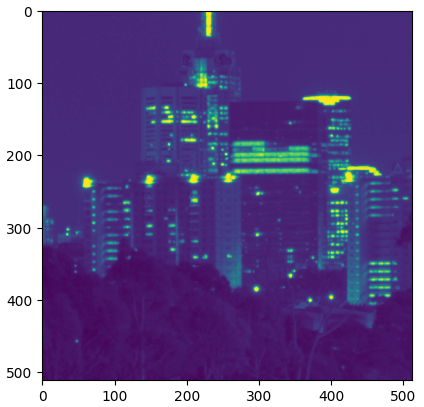
\includegraphics[width=\linewidth]{init.PNG}
                    \caption{Исходное изображение}\label{fig:awesome_image1}
            \end{figure}
        \end{column}
        \begin{column}{0.245\textwidth}
            \begin{figure}
                \centering
                    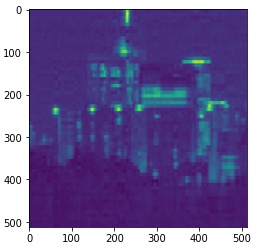
\includegraphics[width=\linewidth]{4.PNG}
                    \caption{96\% сжатие}\label{fig:awesome_image1}
            \end{figure}
        \end{column}
        \begin{column}{0.245\textwidth}
            % \begin{figure}
            %     \centering
            %         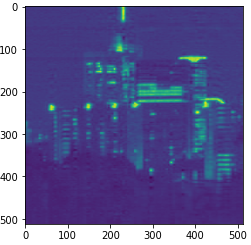
\includegraphics[width=\linewidth]{9.PNG}
            %         \caption{91\% сжатие}\label{fig:awesome_image1}
            % \end{figure}
        \end{column}
        \begin{column}{0.245\textwidth}
            \begin{figure}
                \centering
                    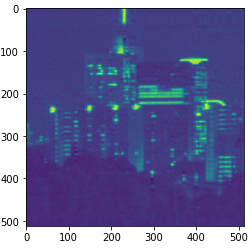
\includegraphics[width=\linewidth]{16.PNG}
                    \caption{84\% сжатие}\label{fig:awesome_image1}
            \end{figure}
        \end{column}
    \end{columns}

\end{frame}

\begin{frame}{Какие были получены результаты?}
    
    \begin{columns}
        \begin{column}{0.47\textwidth}
            \begin{figure}
                \centering
                    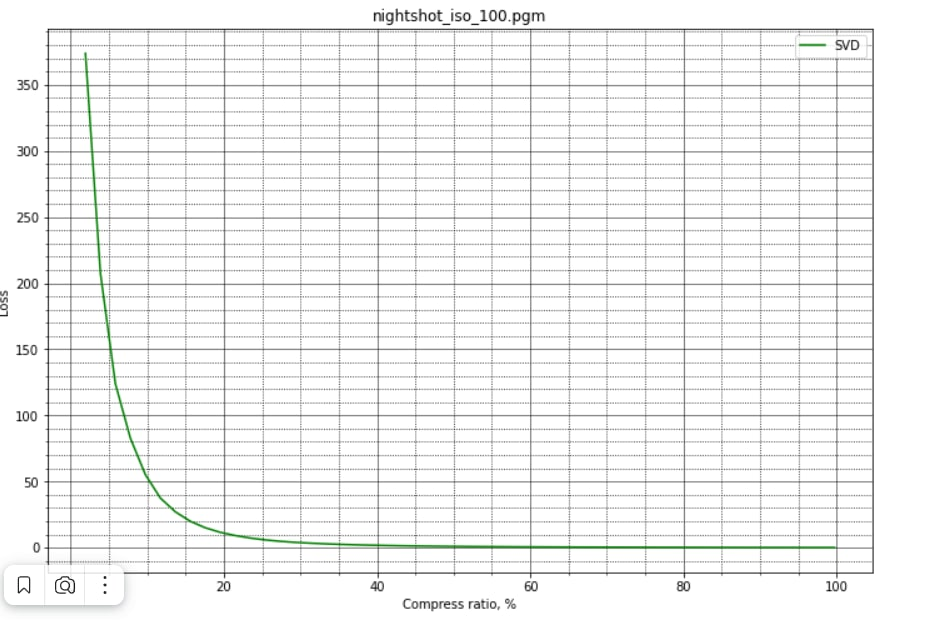
\includegraphics[width=\linewidth]{svd.jpg}
                    \caption{Сжатие SVD}\label{fig:awesome_image1}
            \end{figure}
        \end{column}
        \begin{column}{0.47\textwidth}
            \begin{figure}
                \centering
                    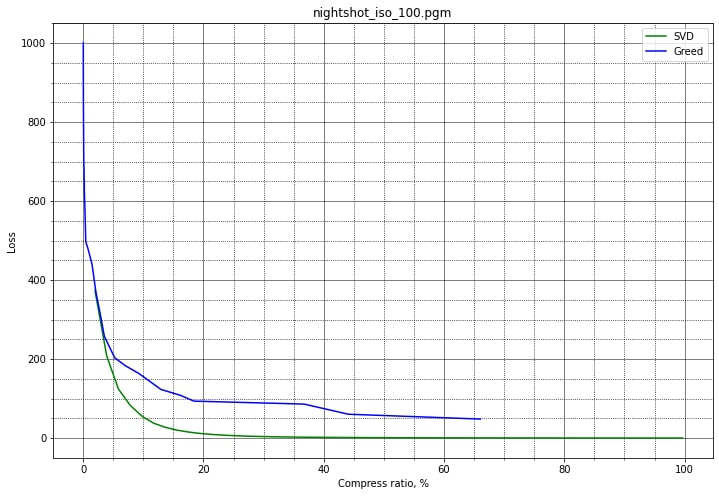
\includegraphics[width=\linewidth]{greed.jpg}
                    \caption{Сжатие алгоритмом из статьи}\label{fig:awesome_image1}
            \end{figure}
        \end{column}
    \end{columns}
        
\end{frame}

\begin{frame}{Что будет дальше?}
\begin{enumerate}
    \item[1)] Освежу в памяти статью \cite{Krumnow2019ComputingEW} 
    \item[2)] Обобщу задачу оптимизации изложенную в статье на тензорные поезда
    \item[3)] Решу полученную задачу
    \item[4)] Проведу численные эксперименты
\end{enumerate}
\end{frame}

\begin{frame}{Источники}
    \bibliographystyle{unsrt}
    \bibliography{biblio}
\end{frame}

\end{document} 
